



\usetikzlibrary{arrows, decorations.markings}

% for double arrows a la chef
% adapt line thickness and line width, if needed


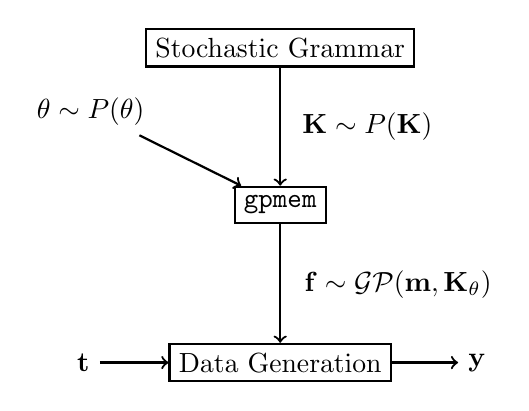
\begin{tikzpicture}[thick]
 \node[draw,rectangle] (grammar) {Stochastic Grammar};
 \node[below left of=grammar,xshift=-1.7cm,yshift=-0.1cm] (theta) {$\bm{\theta} \sim P(\bm{\theta})$};
 \node[draw,rectangle,below of=grammar,yshift=-1cm] (gpmem) {\texttt{gpmem}};
 \node[draw,rectangle,below of=gpmem,yshift=-1cm] (f) {Data Generation};
 \node[below right of=grammar,xshift=0.4cm,yshift=-0.3cm] (k) {$\mathbf{K} \sim P(\mathbf{K})$};
\node[below right of=gpmem,xshift=0.79cm,yshift=-0.3cm] (gp) {$\mathbf{f} \sim \mathcal{GP}(\mathbf{m},\mathbf{K}_{\bm{\theta}})$};
\node[left of=f,xshift=-1.5cm] (x) {$\mathbf{t}$};
\node[right of=f,xshift=1.5cm] (y) {$\mathbf{y}$};

% 1st pass: draw arrows
  \draw[thick,->] (grammar) -- (gpmem);
  \draw[thick,->] (theta) -- (gpmem);
  \draw[thick,->] (gpmem) -- (f);
 \draw[thick,->] (x) -- (f);
 \draw[thick,->] (f) -- (y);
  % Note: If you have no branches, the 2nd pass is not needed
\end{tikzpicture}

